\documentclass[fleqn]{article}
\oddsidemargin 0.0in
\textwidth 6.0in
\thispagestyle{empty}
\usepackage{import}
\usepackage{amsmath}
\usepackage{graphicx}
\usepackage{flexisym}
\usepackage{calligra}
\usepackage{amssymb}
\usepackage{bigints} 
\usepackage[english]{babel}
\usepackage[utf8x]{inputenc}
\usepackage{float}
\usepackage[colorinlistoftodos]{todonotes}


\DeclareMathAlphabet{\mathcalligra}{T1}{calligra}{m}{n}
\DeclareFontShape{T1}{calligra}{m}{n}{<->s*[2.2]callig15}{}
\newcommand{\scriptr}{\mathcalligra{r}\,}
\newcommand{\boldscriptr}{\pmb{\mathcalligra{r}}\,}

\definecolor{hwColor}{HTML}{533179}

\begin{document}

  \begin{titlepage}

    \newcommand{\HRule}{\rule{\linewidth}{0.5mm}}

    \center

    \begin{center}
      
\includegraphics[height=11cm, width=11cm]{asu.png}
    \end{center}

    \vline

    \textsc{\LARGE Classical Parts/Field/Matter II}\\[1.5cm]

    \HRule \\[0.5cm]
    { \huge \bfseries Problem Set 2}\\[0.4cm] 
    \HRule \\[1.0cm]

    \textbf{Behnam Amiri}

    \bigbreak

    \textbf{Prof: Maulik Parikh}

    \bigbreak

    \textbf{{\large \today}\\[2cm]}

    \vfill

  \end{titlepage}

  \begin{enumerate}
    \item Does the function $f(x,y)=2(x^2+y^2)$ satisfy the two-dimensional Laplace’s equation? Check that the function 
    $g(x, y)=x^2-y^2$ does. Sketch the latter function, calculate the gradient at the points $(0, 1), ~ (1, 0), ~ (0, -1),$ 
    and $(-1, 0)$  and indicate by little arrows the directions in which these gradients point. Within the square bounded by the lines $x=\pm 1$ and $y=\pm 1$, where is $g$
    maximum and where is it a minimum? What do you notice about the location of these points that is characteristic of solutions to Laplace’s equation?

      \textcolor{hwColor}{
        \\
        We know that Laplace's equation is a second-order partial differential equation which in rectangular 
        coordinates is
        $$
          \nabla^2 f=\dfrac{\partial^2 f}{\partial x^2}+\dfrac{\partial^2 f}{\partial y^2}+\dfrac{\partial^2 f}{\partial z^2}=0
        $$
        We are given the following functions:
        \\
        \\
        $
          \begin{cases}
            f(x,y)=2(x^2+y^2)
            \\
            \\
            g(x,y)=x^2-y^2
          \end{cases}
        $
        \\
        \\
        \\
        Let's find $\nabla^2 f$ and $\nabla^2 g$
        \\
        \\
        $
          \nabla^2 f=\dfrac{\partial^2}{\partial x^2} \left[2(x^2+y^2)\right]+\dfrac{\partial^2 f}{\partial y^2} \left[2(x^2+y^2)\right]
          =2 \dfrac{\partial }{\partial x} \left[2x\right]+2\dfrac{\partial}{\partial y} \left[2y\right]
          =4+4
          \\
          \\
          \\
          \therefore ~~~ \nabla^2 f=4 \neq 0 ~~~~ \checkmark
          \\
          \\
          \\
          \nabla^2 g=\dfrac{\partial^2}{\partial x^2} \left(x^2-y^2\right)+\dfrac{\partial^2}{\partial y^2} \left(x^2-y^2\right)
          =\dfrac{\partial }{\partial x} \left(2x\right)+\dfrac{\partial }{\partial y} \left(-2y\right)
          =2-2
          \\
          \\
          \\
          \therefore ~~~ \nabla^2 g=0 ~~~~ \checkmark
        $
        \\
        \\
        So far we see that function $f$ does not satisfy the two-dimensional Laplace’s equation and function $g$ satisfies the 
        two-dimensional Laplace’s equation.
        \\
        Here is a sketch for the latter function.
        \\
        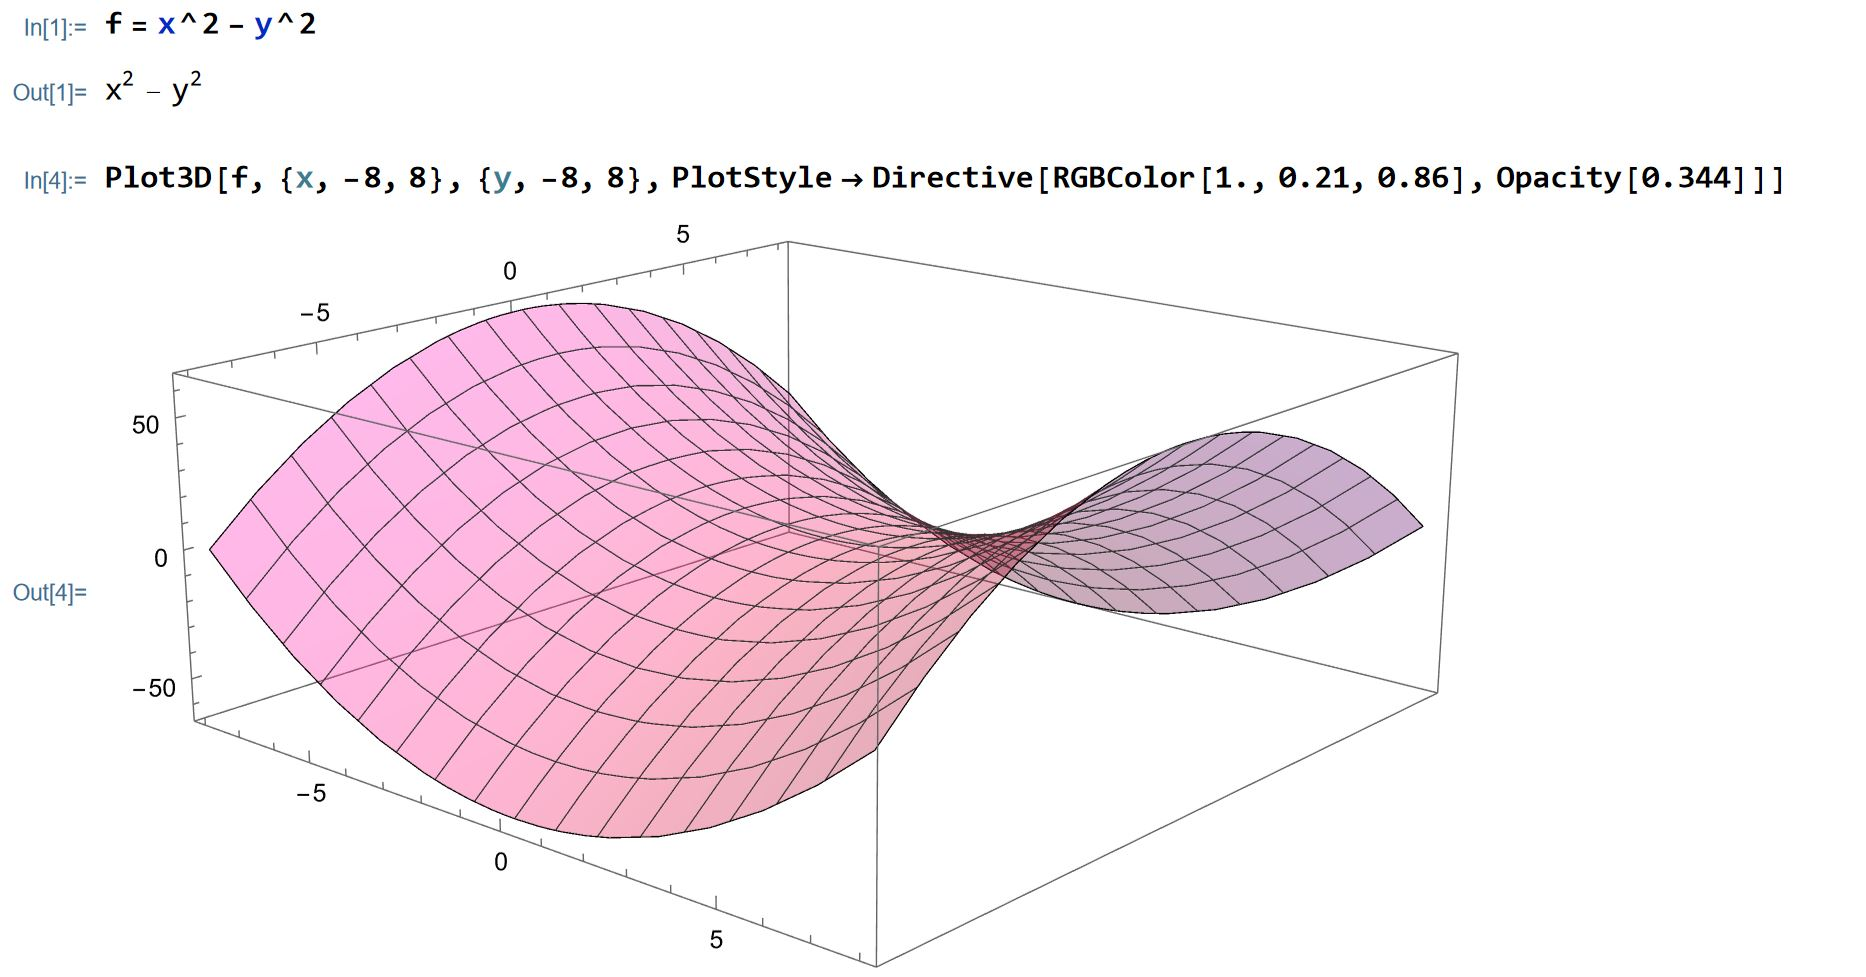
\includegraphics[height=7cm, width=12cm]{One.JPG}
        \\
        \\
        and here is the gradient:
        \\
        \\
        $
          \nabla g=\dfrac{\partial g}{\partial x} ~ \hat{x}+\dfrac{\partial g}{\partial y} ~ \hat{y}
          =\dfrac{\partial}{\partial x} \left(x^2-y^2\right) ~ \hat{x}+\dfrac{\partial}{\partial y} \left(x^2-y^2\right) ~ \hat{y}
          \\
          \\
          \\
          \therefore ~~~ \nabla g=2x ~ \hat{x}-2y ~ \hat{y} ~~~~ \checkmark
        $
        \\
        \\
        We are asked to calculate the gradient at points $(0, 1), ~ (1, 0), ~ (0, -1), ~ (-1, 0)$:
        \\
        \\
        $
          \begin{cases}
            \text{At} ~ (0, 1), ~~ \nabla g(x,y)=2(0) ~ \hat{x}-2(1) ~ \hat{y}=-2 ~ \hat{y}
            \\
            \\
            \text{At} ~ (1, 0), ~~ \nabla g(x,y)=2(1) ~ \hat{x}-2(0) ~ \hat{y}=2 ~ \hat{x} 
            \\
            \\
            \text{At} ~ (0, -1), ~~ \nabla g(x,y)=2(0) ~ \hat{x}-2(-1) ~ \hat{y}=2 ~ \hat{y}
            \\
            \\
            \text{At} ~ (-1, 0), ~~ \nabla g(x,y)=2(-1) ~ \hat{x}-2(0) ~ \hat{y}=-2 ~ \hat{x}
          \end{cases} \Longrightarrow 
          \begin{cases}
            (0, 1) \rightarrow \nabla g(x,y)=(0, -2)
            \\
            \\
            (1, 0) \rightarrow \nabla g(x,y)=(2, 0)
            \\
            \\
            (0, -1) \rightarrow \nabla g(x,y)=(0, 2)
            \\
            \\
            (-1, 0) \rightarrow \nabla g(x,y)=(-2, 0)
          \end{cases}
        $
        \\
        \\
        \\
        The gradient function gives the slope of a function at any single point on its curve. 
        \\
        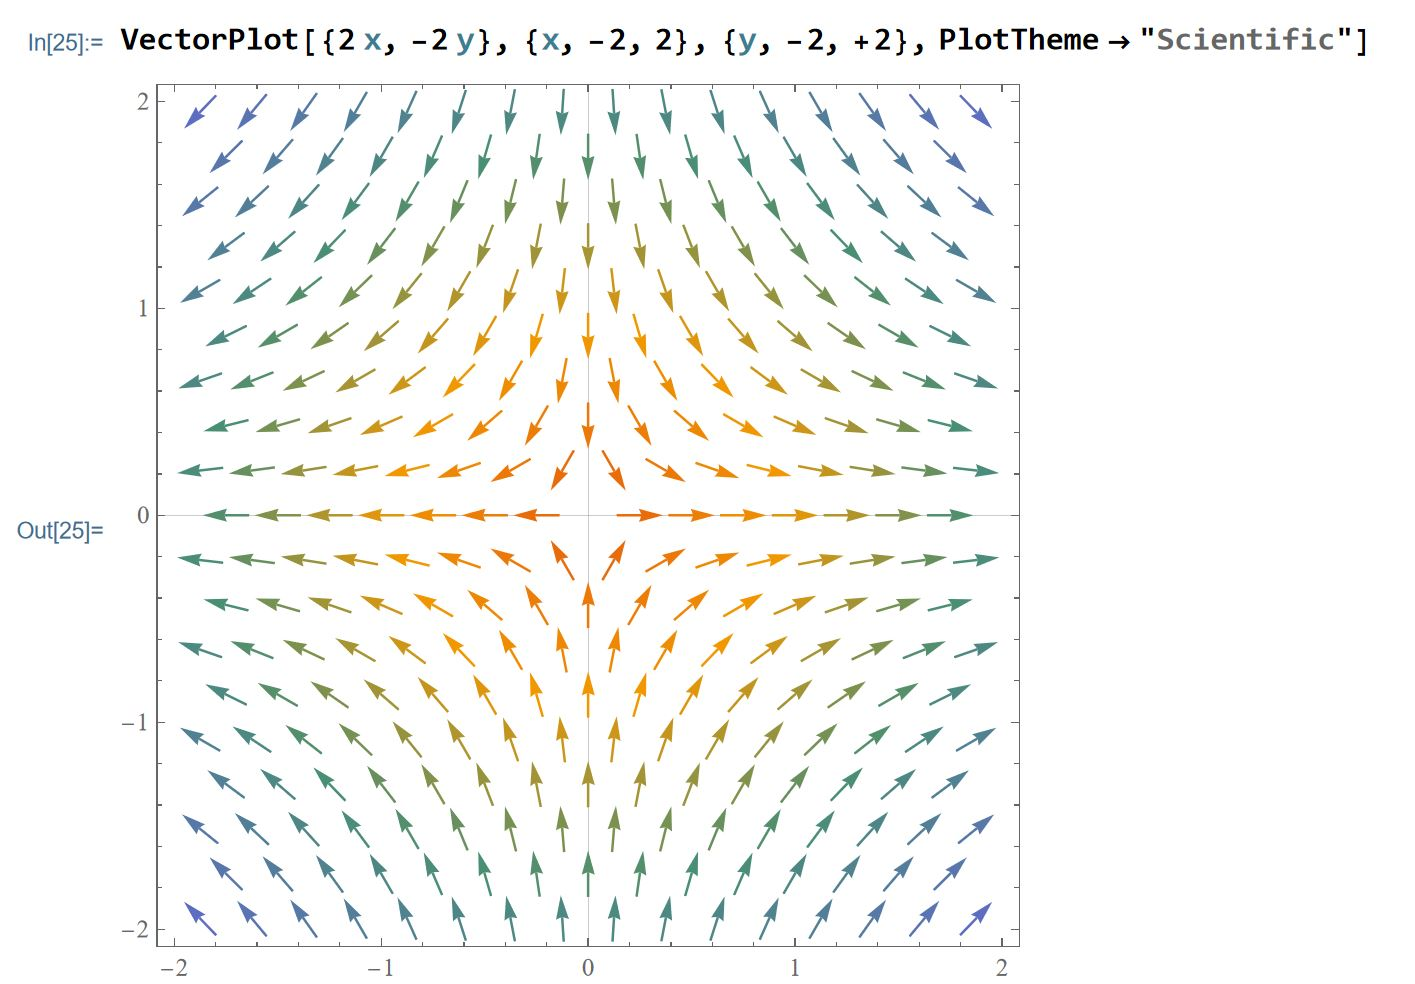
\includegraphics[height=10cm, width=14cm]{Two.JPG}
        \\
        \\
        Above is the direction of the gradient vectors. Now based on the plot we can state that:
        \begin{itemize}
          \item For $(0, 1)$ the direction is downward.
          \item For $(1,0)$ the direction is to the right.
          \item For $(0,-1)$ the direction is upward.
          \item For $(-1,0)$ the direction is to the left.
        \end{itemize}
      }

      \textcolor{hwColor}{
        We learned from the textbook that Laplace’s equation tolerates \emph{no local maxima or minima}. Extreme values must 
        occur at the boundries. \emph{If a continuous function $f$ has no local extrema in the interior of a closed region 
        $\mathbb{R}^2$, then its maximal and minimal values on $R$ must occur on the boundary of $R$.} Since our boundry is the 
        square then the maxima must occur in the sqaure.
        \\
        \\
        $\forall ~ x,y \in \mathbb{R}, ~ x^2 ~ \text{and} ~ y^2 \in \mathbb{R}^+$ therefore,
        \\
        \begin{itemize}
          \item When $x=0$ then $x^2-y^2$ is at its min. $(0, -1), (0, 1)$.
          \item When $y=0$ then $x^2-y^2$ is at its max. $(-1, 0), (1, 0)$.
        \end{itemize}
      }

      \textcolor{hwColor}{
        The location of these points are on the boundry which is an interesting fact.
        \\
      }

    \item A charge $q$ is placed at the origin, exactly between two parallel grounded conducting infinite $x−y$ planes, which are separated by a 
    distance $2d$ in the $z$-direction (so the charge is a distance $d$ away from each plane). Suppose we are interested in the region 
    between the conducting planes, $−d < z < d$. Determine the charges and locations of the image charges
    that would allow us to do away with the conducting planes.

      \textcolor{hwColor}{
        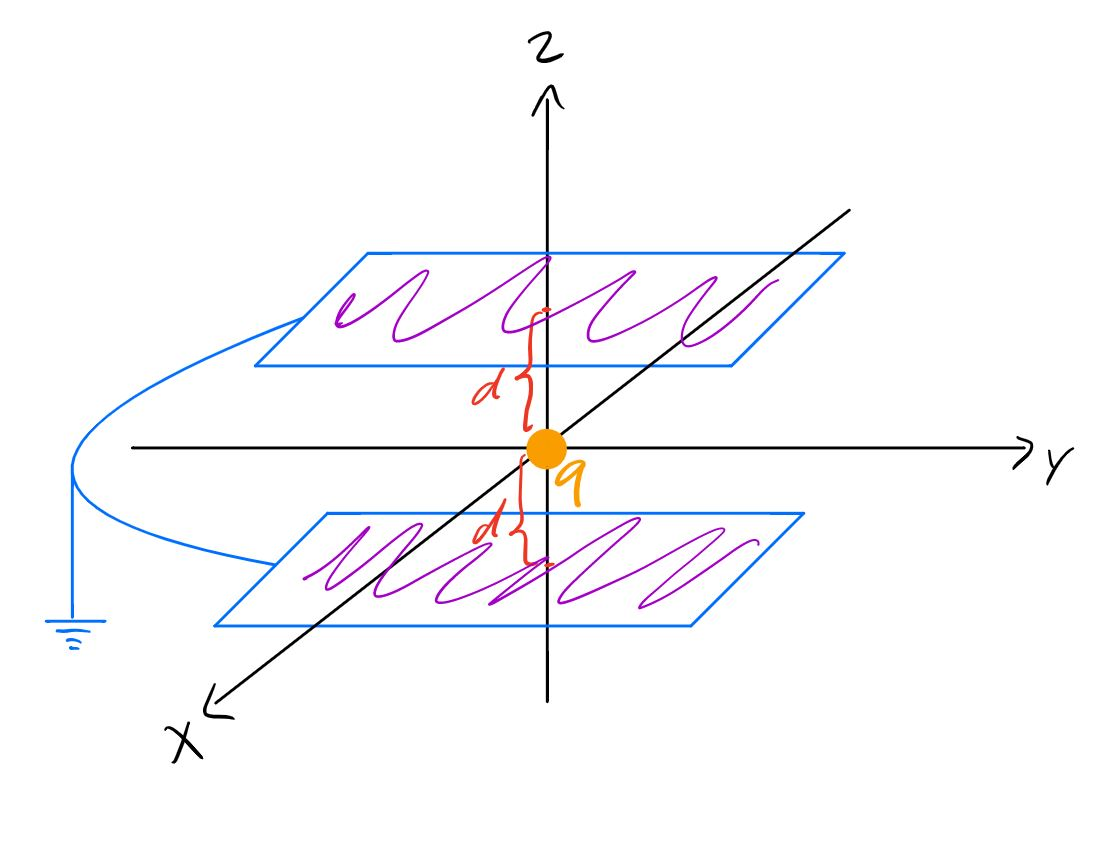
\includegraphics[height=6cm, width=10cm]{Three.JPG}
        \\
        We use \emph{the method of images} for this problem. We have two infinite planes metal parallel to the $x-y$ plane. A point charge $q$ is located
        at the origin. The boundary conditions for this configuration are:
        \begin{itemize}
          \item $V=0$ when $z=d$. (since the conducting planes are grounded)
          \item $V \to 0$ far from the charge that is $x^2+y^2+z^2 >>> d^2$.
        \end{itemize}
        Let's now imagine a totally new configuration that looks like this:
        \\
        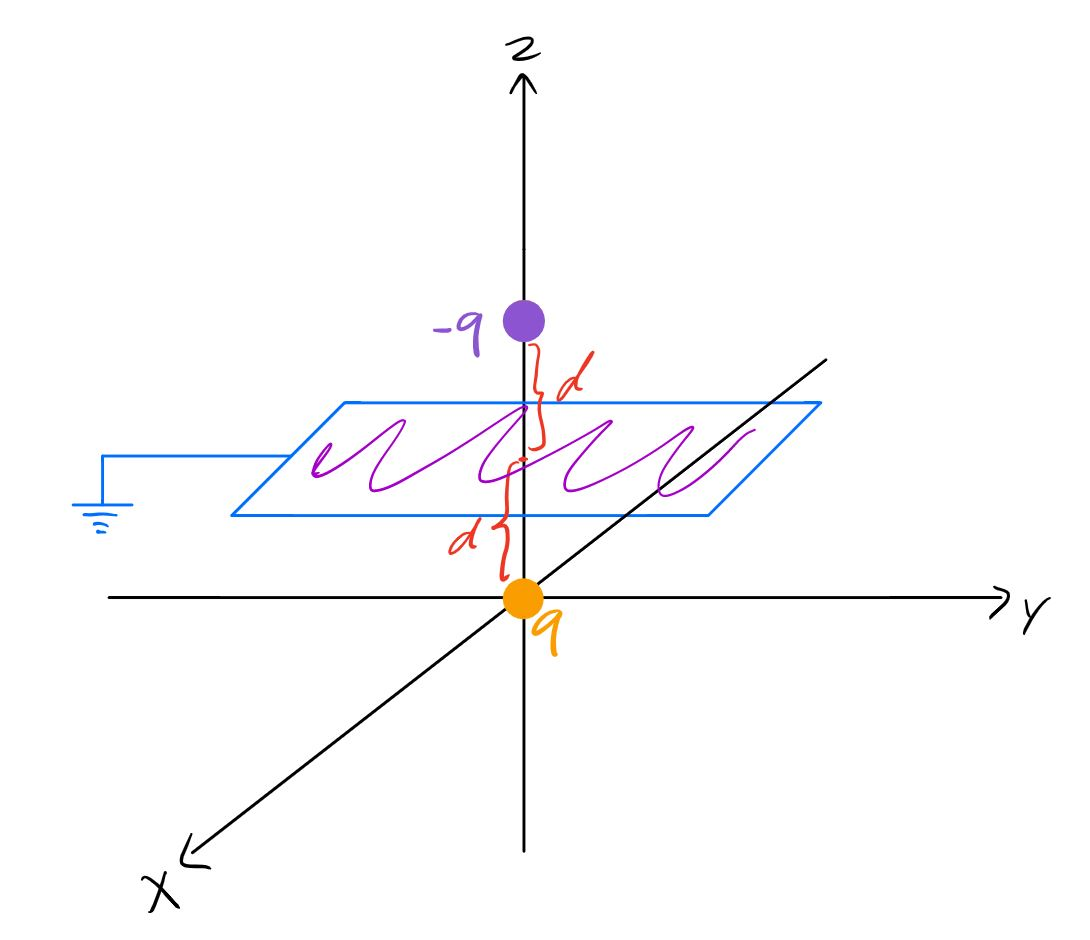
\includegraphics[height=6cm, width=10cm]{Four.JPG}
        \\
        The image charge is placed a distance $d$ above the plane. This will cause a zero potential along the entire $x-y$ plane located at $z=d$. In such
        problems, we first need to determine the boundary conditions.
        \begin{itemize}
          \item $V=0$ at $z=d$.
          \item $V \to 0$ far from the charge that is $x^2+y^2+z^2 >>> d^2$.
        \end{itemize}
        Hence, the potential in the region below the plane is given by the superposition of the potential of the charge $q$ and the
        image charge $-q$. To find $V(x, y, z)$ for $z<d$.
        \\
        $
          q=(0, 0, 0), ~~ -q=(0, 0, 2d)
          \\
          \\
          V(x, y, z)=\dfrac{1}{4 \pi \epsilon_0} \left[
            \dfrac{q_1}{\sqrt{(x-x_0)^2+(y-y_0)^2+(z-z_0)^2}}
            +\dfrac{q_2}{\sqrt{(x-x_0)^2+(y-y_0)^2+(z-z_0)^2}}
          \right]
          \\
          \\
          \\
          =\dfrac{1}{4 \pi \epsilon_0} \left[
            \dfrac{+q}{\sqrt{(x-0)^2+(y-0)^2+(z-0)^2}}
            +\dfrac{-q}{\sqrt{(x-0)^2+(y-0)^2+(z-2d)^2}}
          \right]
          \\
          \\
          \\
          \therefore ~~~ V(x, y, z)=\dfrac{1}{4 \pi \epsilon_0} \left[
            \dfrac{+q}{\sqrt{x^2+y^2+z^2}}
            +\dfrac{-q}{\sqrt{x^2+y^2+(z-2d)^2}}
          \right] ~~~~ \checkmark
        $
        \\
        \\
        So now that we determined what the potential is for the second configuration, we can check it with our previous 
        boundary conditions. Our previous boundry condition said 
        \begin{itemize}
          \item (A) ~~~ $V=0$ when $z=d$ and $z=-d$ (since the conducting planes are grounded) 
          \item (B) ~~~ $V \to 0$ far from the charge that is $x^2+y^2+z^2 >>> d^2$. 
        \end{itemize}
        \textbf{Checking (A):}
        \\
        \\
        $
          V(x, y, z)=\dfrac{1}{4 \pi \epsilon_0} \left[
            \dfrac{+q}{\sqrt{x^2+y^2+d^2}}
            +\dfrac{-q}{\sqrt{x^2+y^2+(d-2d)^2}}
          \right]=0
        $
        \\
        \\
        Well the first condition (A) is satisfied.
        \\
        \\
        \textbf{Checking (B):}
        \\
        \\
        $
          V(x, y, z)=\dfrac{1}{4 \pi \epsilon_0} \left[
            \dfrac{+q}{\sqrt{x^2+y^2+z^2}}
            +\dfrac{-q}{\sqrt{x^2+y^2+z^2}}
          \right]=0 ~~~ \textbf{As $x^2+y^2+z^2 >> d^2$}
        $
        \\
        \\
        By comparing the two configurations we can tell that they both have the exact same boundary conditions. And since 
        the potential we found satisfies both boundary conditions, according to the first uniqueness theorem, $V$ must be 
        the exact same potential for the first setup as well.
        \\
        \\
        Time to study the locations of the image charges. We need an infinite number of charges $\pm q$ located at increasing
        distances on the $z$ axis. Let's start by putting $-q$ at $(0, 0, 2d)$. This charge insures the upper conducting plane
        has a zero potential. Now the lower plane is no longer an equipotential due to the two charges. We can place two other 
        charges at $-2d$ and $-4d$ to make the lower plane an equipotential. But there is an issue now! The upper plane is no longer
        an equipotential. Therefore, we can add two more charges on the top of the upper plane. We keep adding pairs of 
        $\pm q$ image charges at distances further and further away from the two planes. 
        \\
        \\
        The farther the image charges are from the conducting planes, the less they will contribute to the potential in 
        the space between the plates.
        \\
        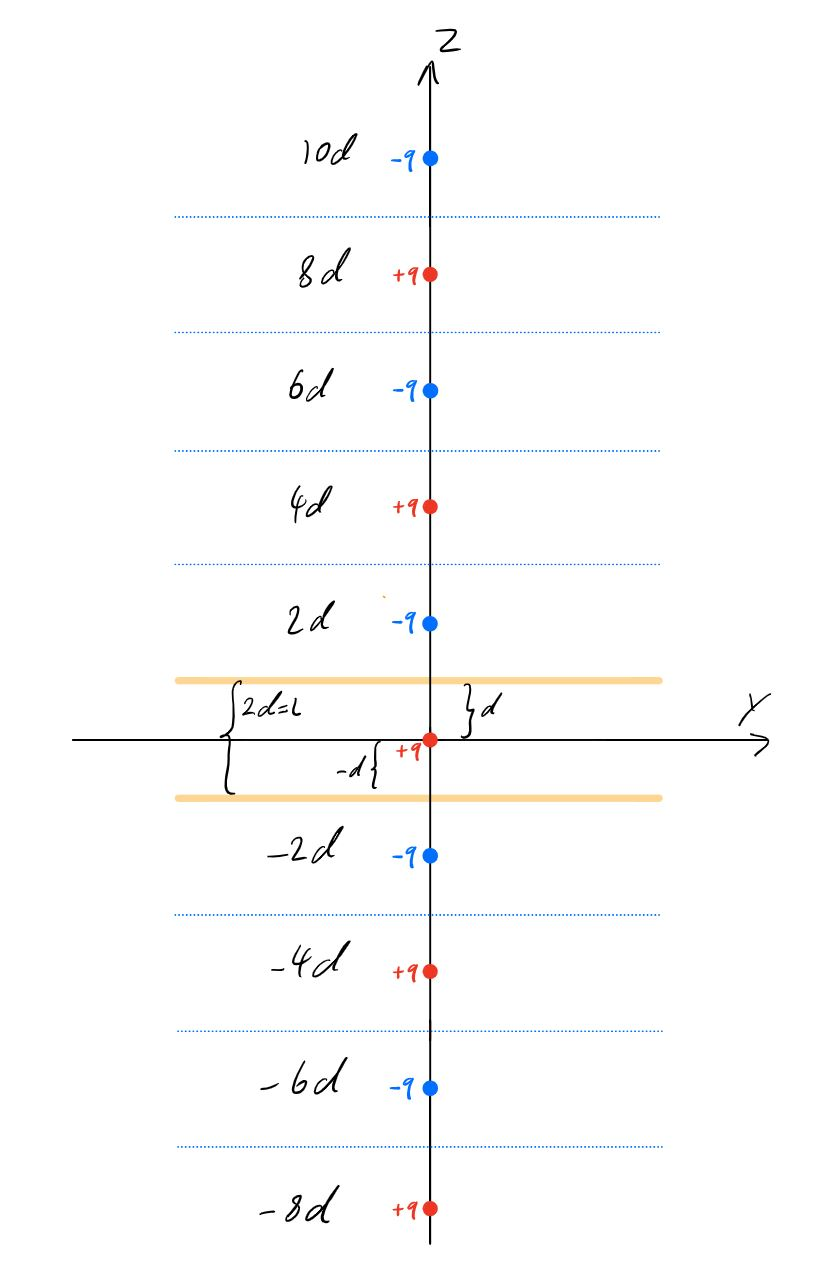
\includegraphics[height=14cm, width=10cm]{Five.JPG}
        \\
      }

    \pagebreak

    \item We want to design a spherical capacitor with an outer conducting shell of given radius $R_2$ and an inner conducting sphere of 
    unknown radius $R_1$. Suppose we want our capacitor to store the maximum possible energy subject to the constraint that the electric 
    field at the surface of the inner sphere not exceed $E_0$. Find the radius $R_1$ for the inner sphere as well as the total amount of 
    electrical energy stored in the capacitor.

      \textcolor{hwColor}{
        \\
        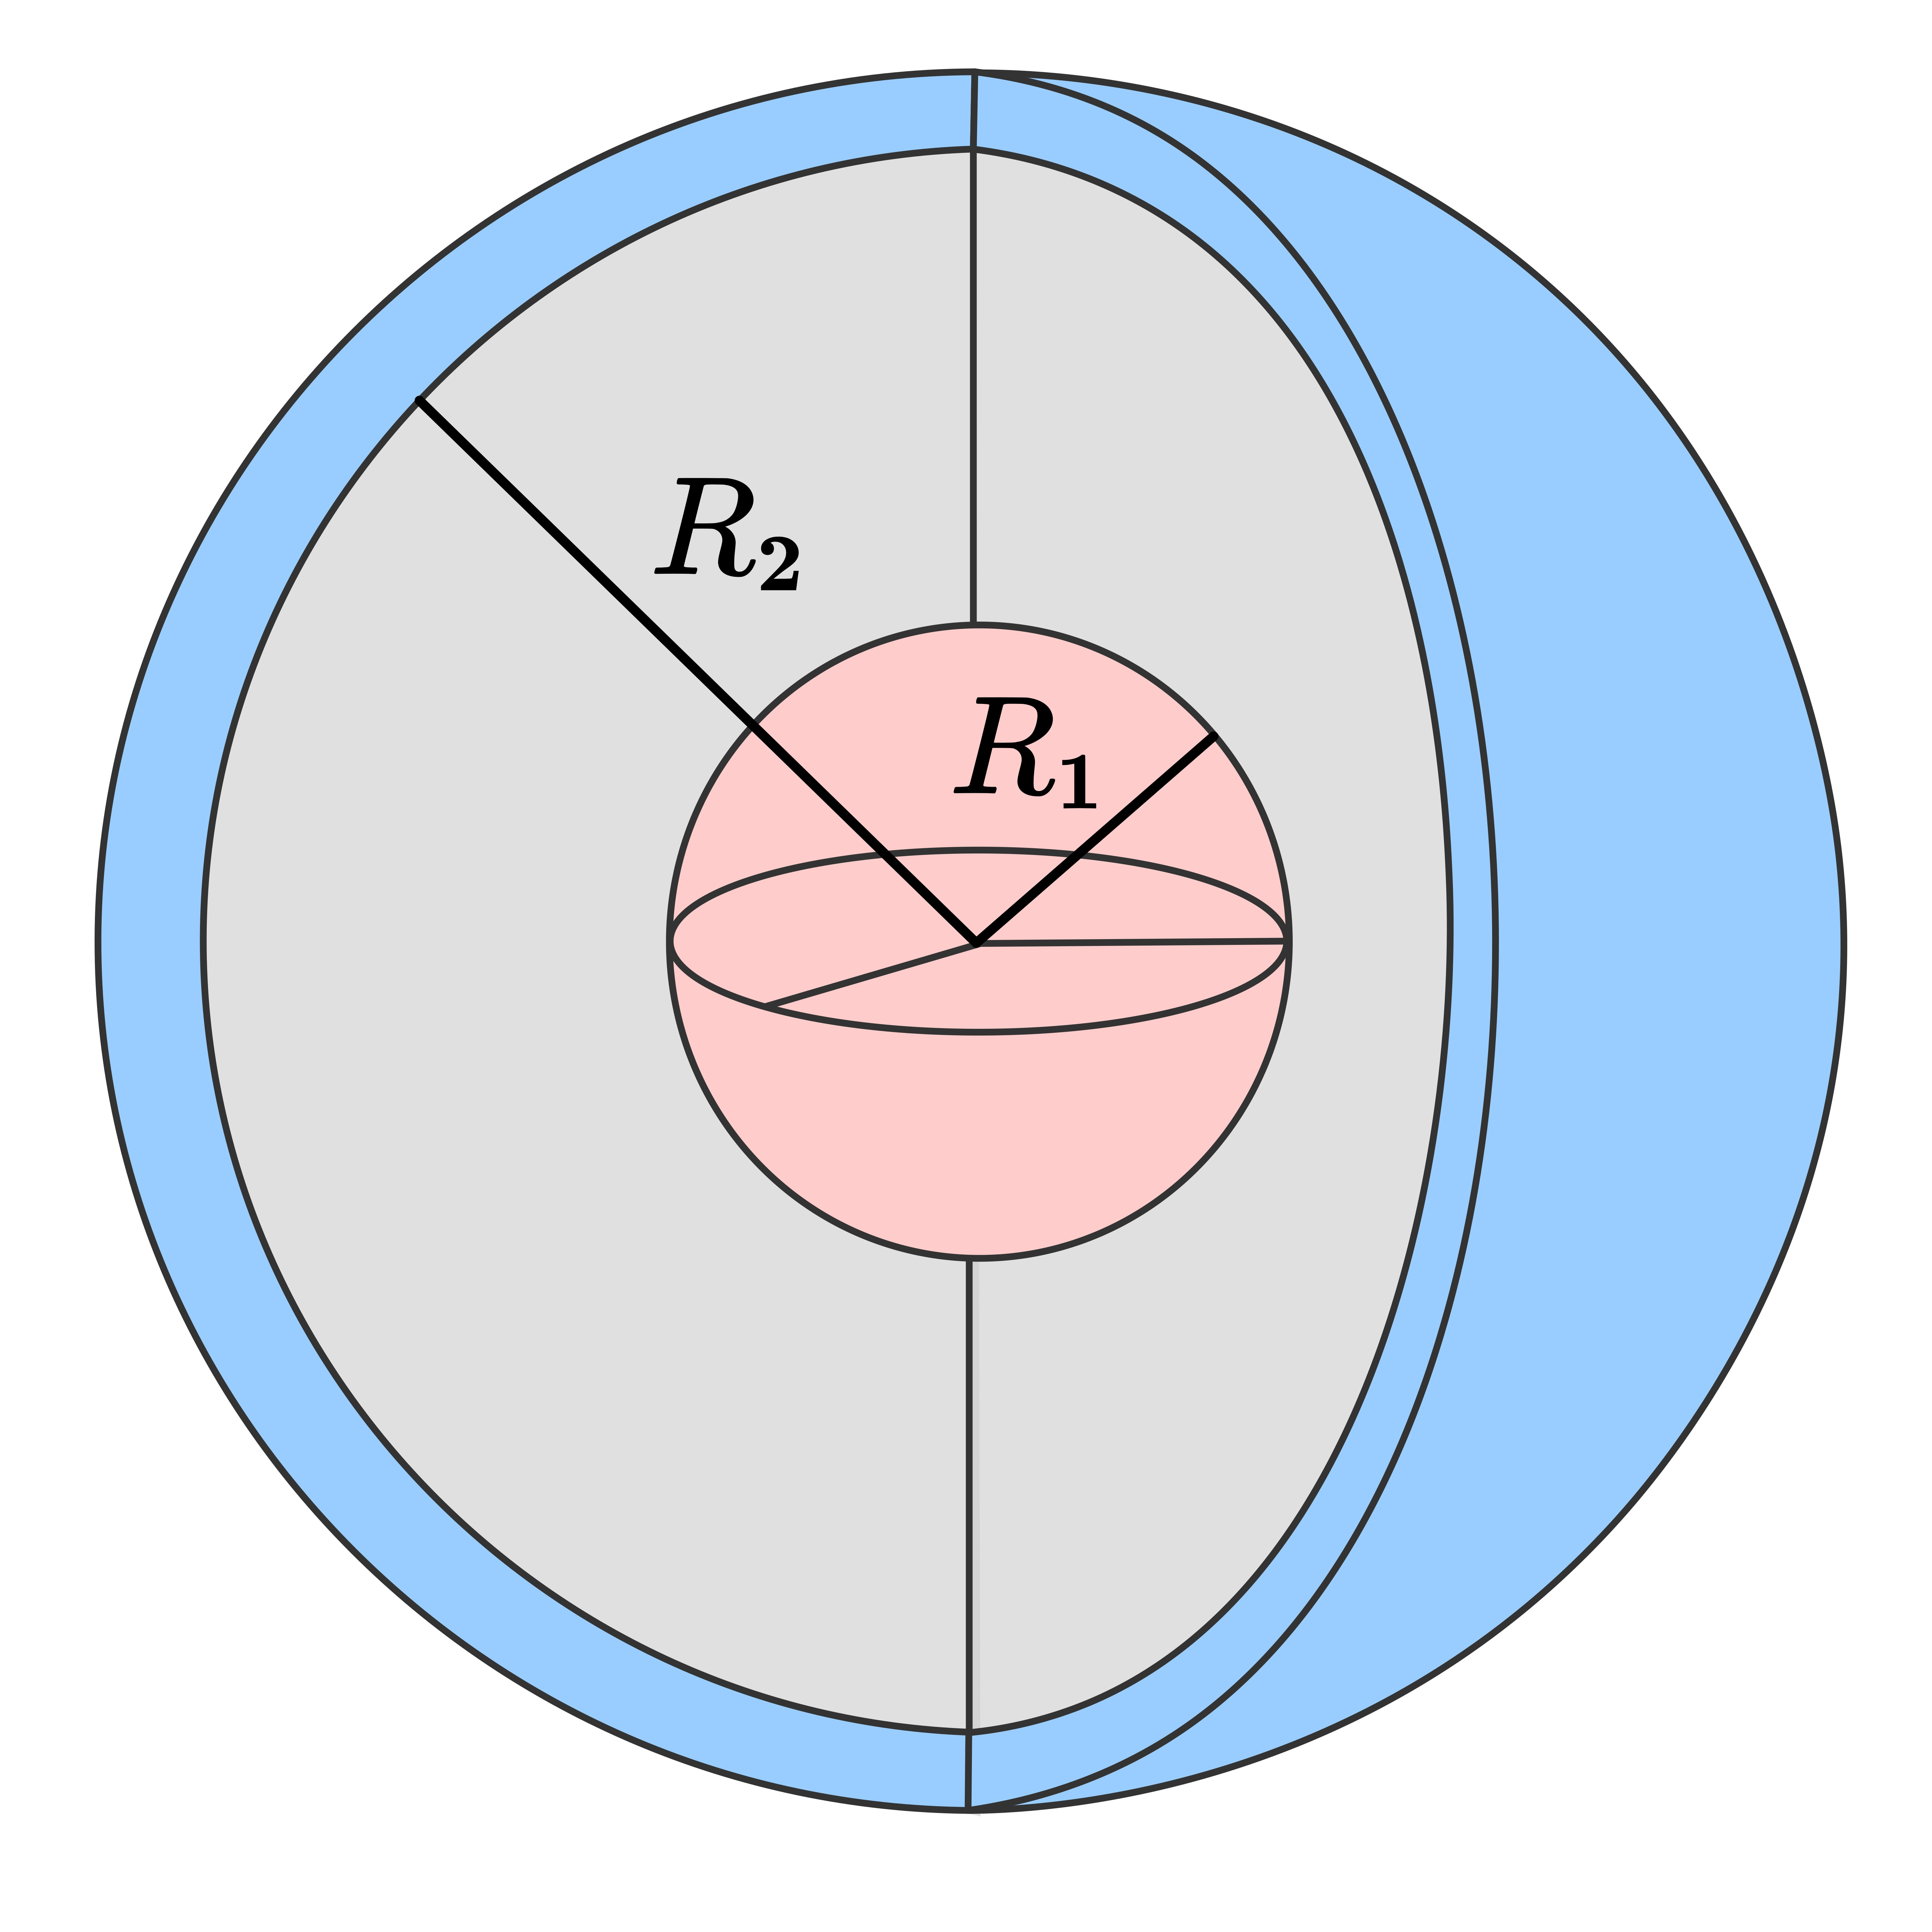
\includegraphics[height=7cm, width=7cm]{Six.jpg}
        \\
        The two shells are charged so the inner shell has $+q$ charge and the outter one has $-q$ charge.
        Recall that Gauss's law states that the electric flux through a closed surface equals total enclosed charge divided 
        by electrical permittivity of vacuum. 
        $$
          \phi=\bigoint\limits_{Surface} \overrightarrow{E} . d\overrightarrow{a}=\dfrac{1}{\epsilon_0} Q_{enclosed}
        $$
        By imagining a spherical surface (Gaussian sphere) between the two shells with radius $r$ we can calculate $\overrightarrow{E}$:
        \\
        \\
        $
          \bigoint\limits_{Surface} \overrightarrow{E} . d\overrightarrow{a}=\dfrac{1}{\epsilon_0} Q_{enclosed}
          \\
          \\
          \\
          \bigints\limits_{Surface} |E| da=\dfrac{1}{\epsilon_0} q \Longrightarrow |E| ~ 4 \pi r^2=\dfrac{1}{\epsilon_0} q
          \\
          \\
          \\
          \therefore ~~~ \overrightarrow{E}=\dfrac{1}{4 \pi \epsilon_0} \dfrac{q}{r^2} \hat{r} ~~~~ R_1<r<R_2 ~~~~ \checkmark
        $ 
        \\
        \\
        Now we are set to find the potential differnce between the two shells. On page 105 of the textbook we learned how to find the potential 
        difference between them.
        \\
        \\
        $
          V=V_+-V_-=-\bigints\limits_{(-)}^{(+)} \overrightarrow{E} . d\overrightarrow{a}
          =\bigints\limits_{(+)}^{(-)} \overrightarrow{E} . d\overrightarrow{a}
          \\
          \\
          \\
          =\bigints\limits_{R_1}^{R_2} \left(\dfrac{1}{4 \pi \epsilon_0} \dfrac{q}{r^2} \hat{r}\right).d\overrightarrow{a}
          =\dfrac{q}{4 \pi \epsilon_0} ~~ \bigints\limits_{R_1}^{R_2} \dfrac{1}{r^2} \hat{r}.d\overrightarrow{r}
          \\
          \\
          \\
          =\dfrac{q}{4 \pi \epsilon_0} ~~ \bigints\limits_{R_1}^{R_2} \dfrac{1}{r^2}  dr
          =\dfrac{q}{4 \pi \epsilon_0} ~~ \dfrac{-1}{r} \Big|_{R_1}^{R_2}
          \\
          \\
          \\
          \therefore ~~~ V=\dfrac{q}{4 \pi \epsilon_0} \left(-\dfrac{1}{R_2}+\dfrac{1}{R_1}\right) ~ > 0
        $
        \\
        \\
        From chapter 2, page 107 we know that the total energy of the system as 
        \\
        \\
        $
          U=\dfrac{1}{2} C V^2=\dfrac{1}{2}Q V=\dfrac{1}{2}\dfrac{Q^2}{C}
        $
        \\
        \\
        We are told that the electric potential does not exceed $E_0$. We already found $E ~~ R_1<r<R_2$. By plugging $E_0$ into it, 
        we have:
        \\
        \\
        $
          |E_0|=\dfrac{1}{4 \pi \epsilon_0} \dfrac{q}{R^2_1}
          \\
          \\
          \therefore ~~~ q=4 \pi \epsilon_0 E_0 R^2_1 ~~~~ \checkmark
        $
        \\
        \\
        Now we can calculate the electrical energy stored in the capacitor subject to the constraint.
        \\
        \\
        $
          U=\dfrac{1}{2} q V
          =\dfrac{1}{2} 
          \left(4 \pi \epsilon_0 E_0 R^2_1\right) 
          \left[\dfrac{q}{4 \pi \epsilon_0} \left(-\dfrac{1}{R_2}+\dfrac{1}{R_1}\right)\right]
          \\
          \\
          \\
          =\dfrac{1}{2} \left(4 \pi \epsilon_0 E_0 R^2_1\right) 
          \left[\dfrac{4 \pi \epsilon_0 E_0 R^2_1}{4 \pi \epsilon_0} \left(-\dfrac{1}{R_2}+\dfrac{1}{R_1}\right)\right]
          \\
          \\
          \\
          =\dfrac{1}{2} \left(4 \pi \epsilon_0 E_0 R^2_1\right) 
           \times E_0 R^2_1 \left(\dfrac{-R_1+R_2}{R_1 R_2}\right)
          \\
          \\
          \\
          \therefore ~~~ U=2 \pi \epsilon_0 ~ \dfrac{E^2_0 R^3_1}{R_2} \left(-R_1+R_2\right) ~~~~ \checkmark
        $
        \\
        \\
        We know from calculus that by equating the first derivative to zero we can find maxima and minima. By setting the first derivative 
        of $U$ with respect to $R_1$ we can calculate the radius $R_1$ to store the maximum possible energy.
        \\
        \\
        $
          \dfrac{dU}{dR_1}=\dfrac{d}{dR_1} \left[2 \pi \epsilon_0 ~ \dfrac{E^2_0 R^3_1}{R_2} \left(-R_1+R_2\right)\right]
          \\
          \\
          \\
          =2 \pi \epsilon_0 \dfrac{E^2_0}{R_2} \dfrac{d}{dR_1} \left[-R^4_1+R^3_1 R_2\right]
          =2 \pi \epsilon_0 \dfrac{E^2_0}{R_2} \left(-4 R^3_1+ 3 R^2_1 R_2\right)
          =2 \pi \epsilon_0 \dfrac{E^2_0 R^2_1}{R_2} \left(-4R_1+ 3R_2\right)
          \\
          \\
          \\
          \dfrac{dU}{dR_1}=0 \Longrightarrow 2 \pi \epsilon_0 \dfrac{E^2_0 R^2_1}{R_2} \left(-4R_1+ 3R_2\right)=0
          \\
          \\
          \\
          \therefore ~~~ -4R_1+ 3R_2=0 
          \\
          \\
          \\
          \therefore ~~~ R_1=\dfrac{3}{4} R_2 ~~~~ \checkmark
        $
        \\
        \\
        We are almost done. Time to calculate the total amount of electrical energy stored in the capacitor.
        \\
        \\
        $
          U=2 \pi \epsilon_0 ~ \dfrac{E^2_0 \left(\dfrac{3}{4} R_2\right)^3}{R_2} \left[-\left(\dfrac{3}{4} R_2\right)+R_2\right]
          =2 \pi \epsilon_0 ~ \dfrac{E^2_0 \dfrac{27}{64} R^3_2}{R_2} \left[\dfrac{1}{4}R_2\right]
          \\
          \\
          \\
          \therefore ~~~ U=2 \pi \epsilon_0 \dfrac{27 E^2_0 ~ R^3_2}{256} ~~~~ \checkmark
        $
        \\
      }

    \pagebreak

    \item Is the following argument correct? Explain in detail. A point charge $q$ is located at an off-center position inside an 
    uncharged conducting spherical shell. We know the potential must be constant on the inner surface of the shell. Therefore, by the 
    uniqueness theorem, the potential is constant in the hollow interior as well. Hence the electric field inside is zero and the 
    charge therefore experiences no force.

      \textcolor{hwColor}{
        \\
        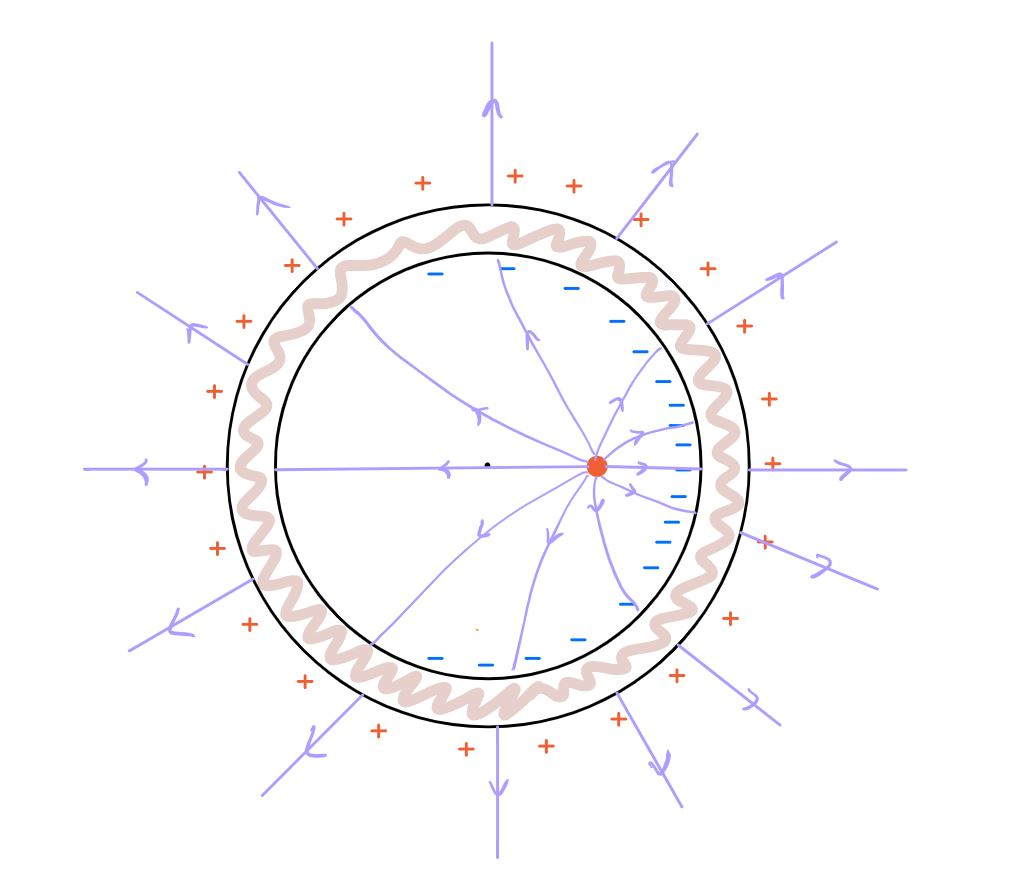
\includegraphics[height=5cm, width=7cm]{Seven.JPG}
        \\
        The offset charge produces a non-spherically symmetric field. This field in turn induces a non-spherically symmetric charge distribution 
        on the internal surface. But the charge to create this field has to come from somewhere. There is no effect of the interior charge 
        and the inner induced charge in all space beyond the inner surface. It effectively doesn't exist. But the charge accumulated on 
        the interior surface had to come from some where. There were random changes in the previously neutral charge distribution within 
        the volume. These charges affect each other even though they aren't effected by charges closer to the center. If you place charge
        in a conductor, it will distribute itself evenly on the outer surface seeking to minimize the potential energy.
        \\
        With the help of the Method of Images we can state that since the electric field is zero within the conductor, the electric potential is constant within
        the conductor. We only care about differences in potential, so we can call this potential zero. Given our internal charge, we can calculate 
        the electric potential on the inner surface due to the internal charge. Now consider an infinite line from the center of the sphere 
        through the internal charge. Where on this line do we need to put a new charge so that its potential plus the potential of the internal 
        charge is zero at the points where the line intersects the internal surface? We have an equation at each point of intersection. Our 
        equations will have two unknowns. Solve the equations for two unknowns and we will know where on the line to place the charge and how much
        charge to put. Now calculate the electric field due to the placement of this Image Charge and the original charge and we have the field 
        due to the original charge and the real induced charge. In some ways a point charge is equivalent to the induced charge.
        \\
        \begin{itemize}
          \item $E=0$ inside conducting shell.
          \item Charge density induced on inner surface non-uniform.
          \item Charge density induced on outer surface uniform.
          \item $E$ outside has spherical symmetry centered on spherical conducting shell.
        \end{itemize}
      }


    \item A point charge $−2q$ is placed at the origin and a point charge $3q$ is
    place on the $z$-axis at $(0, 0, b$). Calculate
    \begin{enumerate}
      \item The monopole moment.
 
        % \textcolor{hwColor}{

        % }


      \item The dipole moment.

        % \textcolor{hwColor}{

        % }


      \item And the approximate electric potential at large r to order $(1/r2)$
      in spherical coordinates.

        % \textcolor{hwColor}{

        % }
      
    \end{enumerate}


    \item A spherical shell has radius $R$ and uniform surface charge density $\sigma$. Find the electric potential 
    at a point on the surface
    \begin{enumerate}
      \item By using the symmetry of the problem.

        % \textcolor{hwColor}{

        % }
      
      \item By brute-force integration using $\rho=\sigma \delta(r-R)$ where $\delta$ is the
      radial Dirac-delta function obeying $\bigints\limits_{0}^{\infty} \delta(r-R)dr=1$

        % \textcolor{hwColor}{

        % }
    \end{enumerate}



    \item An infinite hollow rectangular pipe runs along the $x$-axis from $-\infty < x < \infty$. Suppose that three sides of the pipe 
    (at $y=0$, $z=0$, and $y=a$) are made of metal. If the fourth side (at $z=b$) is kept at the constant potential $V_0$, find the 
    electric potential inside the pipe.

      % \textcolor{hwColor}{

      % }


    \item A conducting hollow shell of radius $R$ has charge $Q$. We want to know why the shell doesn’t just spontaneously discharge 
    by having its charge go off into the space around it. (For this problem, we’ll think in terms of classical electrostatics, 
    ignoring the atomic structure of the conductor.) Suppose we try to peel off a charge q. Charge conservation
    says that $Q−q$ remains on the shell. Calculate the potential energy (not electric potential) for the removed charge as a 
    function of distance $r$ from the center of the shell (for $r > R$). Be sure to take into account both the remaining charge on 
    the shell and the surface charge induced on it by the removed charge q (see Griffiths Example 3.2 for help with
    the corresponding image charge). Show that there is an energy barrier preventing the shell from spontaneously discharging.
  
      % \textcolor{hwColor}{

      % }

  \end{enumerate}

\end{document}